\section{Theory}

XXX intro

Usually, when designing digital circuits, two major simplifications
are made. The first is that the signals are discrete, or digital. The
second simplification is to look at the time as discrete. Theese
simplifications makes it meaningful to talk about momentarily state of
the circuits, namely the contents of memory elements. The concept of
next state is also meaningful, as the whole circuit is synchronized by
a common clock, which also assures correct timing and data validity
across the circuit.

When designing clockless circuits, the second simplification no longer
holds. Technical aspects, like timing and data validity, must be
guaranteed by other means. For the designer, it demands a change in
the reasoning, as it is, in general, no longer meaningful to look at a
momentarily state.

In this section, I will discuss the technical aspects of clockless
design, while design tools for designing will be discussed in
section~\ref{sec:tools}.

The strictest class of clockless circuits, delay insensive (DI)
circuits, assumes only bounded and positive, but unknown, delays in
wires and gates. Such circuits can only be constructed of C-elements
(see Figure~\ref{fig:c}) and inverters. In \cite{dilimit} it is shown
that it is impossible to create any useful circuits with this
methodology. The article suggests the introduction of a timing
assumption to facilitate the construction of useful circuits: The
isochronic fork.

\begin{figure}[htbp]
  \centering
  \includegraphics{c.pdf}
  \caption{a) Symbol for a C-element, originally designed by David
    E. Muller. b) Truth-table c) Karnough-map d) Gate-level
    implementation. The C-element is the basis of many clockless
    constructs.}
  \label{fig:c}
\end{figure}

An isochronic fork is a timing assumption that requires a signal to be
delivered simultainiously to two circuit elements. This fork allows
the sender of a signal to assume reception with acknowledge from one
of the receivers. The class of circuits depending on isochronic forks
are said to be quasi delay insensitive (QDI), and in \cite{turing} it
is proved that any turing computable function has a QDI
implementation.

\begin{figure}[htbp]
  \centering
  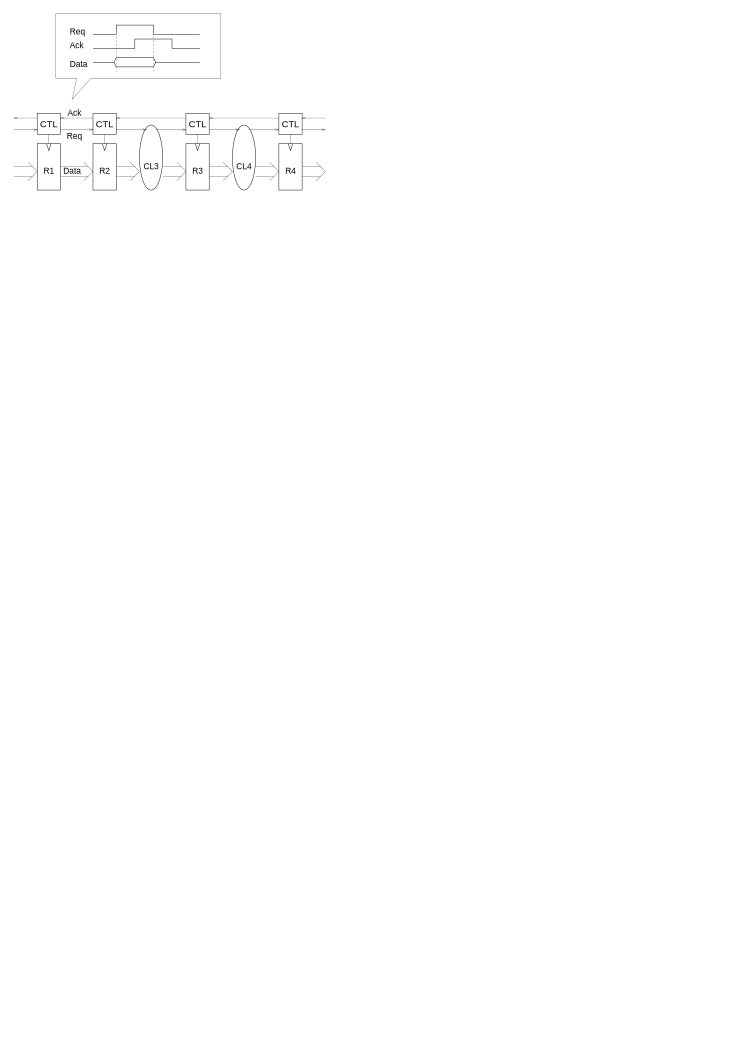
\includegraphics{handshake.pdf}
  \caption{A clockless pipeline implemented with handshaking ensuring
    data validity. Figure from \cite{sparso}.}
  \label{fig:handshake}
\end{figure}

When designing clockless circuits, we need a substitute for the clock
to assure data validity througout the circuit. This can be provided by
handshaking, usually implemented with a variation of the
request-acknowledge protocol as shown in
Figure~\ref{fig:handshake}. The handshaking provides a local clock for
the storage elements, usually latches or C-elements.

There are multiple ways to implement handshaking. This project will
focus XXX on high-level synthesis that is agnostic on the underlying
protocol; even clocked circuits can be synthetisised. 

\subsection{Encodings}

XXX introductory summary of techniques

\begin{figure}[htbp]
  \centering
  \includegraphics{bundled.pdf}
  \caption{Bundled data XXX}
  \label{fig:bundled}
\end{figure}

When using bundled-data, values are represented by conventional
boolean levels, and the handshaking is implemented by bundeling the
request and acknowledge signals with the data as shown in
Figure~\ref{fig:bundled}~a). Bundled data is also refered to as
single-rail, in contrast to dual or N-of-M rail encodings, as data is
encoded as ordinary binary data.

As there usually are no way to determine wether binary data from a
combinatonal function is complete, delays matching the combinational
delay have to be inserted in the control path to maintain correct
behaviour as shown in Figure~\ref{fig:bundeled_delay}.

When using handshake protocols, the handshake can be done in four or
two phases as shown in Figure~\ref{fig:bundled}~b) and c). The four
phase protocol is also referred to as return to zero (RTZ). The two
phase protocol makes better use of the bandwith over the wires, but
usually the four phase protocol is preferred, as it allows for a
simpler implementation consuming less area.

In Figure~\ref{fig:bundled}~a), a \emph{push} channel is shown. This means
that the data source initiates the handshake, as opposed to when the
consumer inititates it. A channel where the consumer initiates the
handshake is referred to as a \emph{pull} channel.

XXX Indication and the muller-C element

If the signal is encoded into a representation using two wires per
bit, one for each value; logic 1 (true) and logic 0 (false). This
redundant representation provides the possibility of a variable to
have an ``empty'' value, also referred to as a NULL. 

\begin{figure}[htbp]
  \centering
  \includegraphics{compdet.pdf}
  \caption{A memory element with completion detection. Figure from XXX.}
  \label{fig:compdet}
\end{figure}

When implementing combinational functions for dual rail encoding, they
are typically split into two functions analogous to the pull up and
pull down networks in CMOS; one to compute the logic 0 or false value,
and one to compute the logic 1 or true value. Completion is indicated
by one of the signals going high, and allows a completion detector as
shown in Figure~\ref{fig:compdet} to control the memory elements.

XXX figure showing dual rail inverter, a dual-rail gate and a ``truth
table''.

Using dual rail encoding also implies using the four phase protocol
(Figure~\ref{fig:bundled}~b)), as the combinational circuits must
return to the NULL state between values to distinguish successive
values on the channel. Care must therefore not only be taken to avoid
hazards on NULL-to-value transitions, but also on the return-to-NULL
transitions.

Hazards are avoided by adding redundant gates XXX

A more generalized method for encoding, is N of M encodings, where
dual rail is 1 of 2 encoding. In \cite[chapter 9]{nullconv}, multiple
of these encodings are surveyed with regards to resources (i.e. area)
for wires and combinations, and power. An ALU for 1 of 4 encoding are
shown to have good characteristics in terms of power, area and
performance, compared to the dual rail encoding. 

XXX mention Fant advanced pipelining, williams bubbles etc?

\subsection{Summary}

XXX

%\begin{quote}
%A register may input and store a new data token from its predecessor
%if its successor has input and stored the data token that the register
%was previously holding
%\end{quote}

